\chapter{Fermionenmassen: Chiralität, Yukawa-Kopplungen und Majorana-Neutrinos}

\lectureoverview{Zunächst rekonstruieren wir den Higgs-Mechanismus für Eichbosonen in einer Spielzeugtheorie \(U(1)\) und stellen dann die entsprechende Frage für Fermionen. Eine Dirac-Masse mischt links- und rechtsh chirale Felder, doch die schwache Wechselwirkung weist ihnen unterschiedliche Ladungen zu und verbietet deshalb eine nackte Masse. Eine Yukawa-Kopplung an das Higgsfeld respektiert die Symmetrie; sobald das Higgsfeld einen Vakuumerwartungswert annimmt, wird dieselbe Wechselwirkung zu einer Fermionenmasse und zu einer messbaren Higgs--Fermion-Kopplung. Im letzten Teil verfolgen wir diese Logik weiter zu Neutrinomassen, möglichen schweren, ungeschützten Teilchen, kosmischer Strahlung, relativistischer Trägheit und Gravitation.}

Die einleitende Wiederholung soll nicht einfach nur die vorherige Vorlesung wiederholen. Wir brauchen daraus eine Idee in einer Form, die sich auf Fermionen übertragen lässt: Eine Masse entspricht einer von null verschiedenen Energie für eine Anregung bei verschwindendem Impuls. Bei einem Feld bedeutet verschwindender Impuls unendliche Wellenlänge oder eine Verschiebung, die überall gleich ist. Eine Theorie, deren Terme nur Ableitungen enthalten, kann eine gleichförmige Verschiebung nicht erfassen. Ein Term ohne Ableitungen kann das.

\section{Die Geschichte der Eichbosonen in einem Zug}

\subsection{Ableitungsenergie und ein masseloser Vektor}

Das Eichfeld des Modells ist \(A_\mu\), mit der Feldstärke
\begin{equation}
  F_{\mu\nu}
  =\partial_\mu A_\nu-\partial_\nu A_\mu .
  \label{eq:l09-field-strength}
\end{equation}
An der Tafel wird der kinetische Term des Eichfelds schematisch als \(F^2\) angeschrieben. Bei einer üblichen Normierung lautet er
\begin{equation}
  \mathcal L_{\mathrm{gauge}}
  =-\frac14 F_{\mu\nu}F^{\mu\nu}.
  \label{eq:l09-gauge-kinetic}
\end{equation}

\begin{figure}[htbp]
\centering
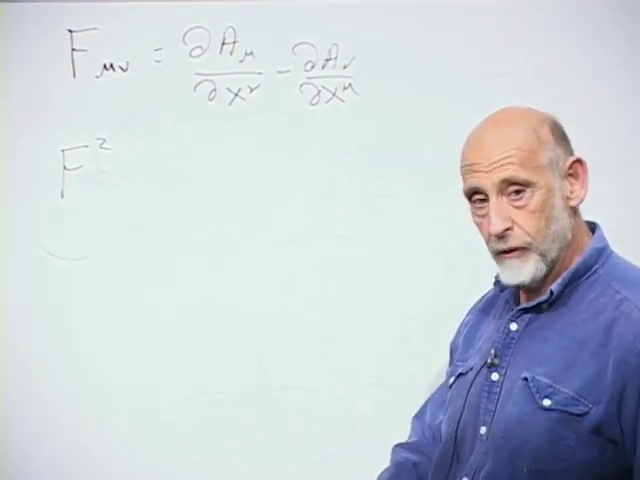
\includegraphics[width=0.72\textwidth]{lecture_09_figure_02.png}
\caption{Definition der Feldstärke und die an der Tafel verwendete Kurzschreibweise \(F^2\) für die Ableitungsenergie des Eichfelds.}
\lectureframe{00:02:39}
\label{fig:l09-field-strength-board}
\end{figure}

Jedes Auftreten von \(A_\mu\) in \eqref{eq:l09-gauge-kinetic} steht unter einer Ableitung. Daher verändert
\begin{equation}
  A_\mu(x)\longmapsto A_\mu(x)+c_\mu,
  \qquad \partial_\nu c_\mu=0,
\end{equation}
\(F_{\mu\nu}\) nicht. Ein homogenes Vektorpotential verursacht folglich keine Feldstärkeenergie. In der Sprache der Vorlesung hat die Mode bei verschwindendem Impuls keine Lücke, und das Eichboson ist masselos.

Dieses \(U(1)\)-Feld ist ein bewusst einfach gehaltener Stellvertreter. Das physikalische Ziel sind \(W^\pm\) und \(Z\), nicht das Photon der Elektromagnetischen Wechselwirkung. Die ungebrochene elektromagnetische Symmetrie lässt das Photon masselos; die gebrochene elektroschwache Symmetrie verleiht den schwachen Eichbosonen eine Masse.

\subsection{Den radialen Freiheitsgrad des Higgsfelds einfrieren}

Führen wir ein geladenes komplexes Skalarfeld ein und schreiben es in Polarkoordinaten:
\begin{equation}
  \phi(x)=\rho(x)e^{i\alpha(x)}.
\end{equation}
Sein mexikanisches-Hut-Potential hat sein Minimum auf einem Kreis mit endlichem Radius. Bezeichnen wir diesen Radius mit \(f\), so ist die radiale Richtung vergleichsweise steif. Für die erste Betrachtung frieren wir sie ein und behalten nur die Phase:
\begin{equation}
  \phi(x)\simeq f e^{i\alpha(x)}.
  \label{eq:l09-frozen-higgs}
\end{equation}

\begin{figure}[htbp]
\centering
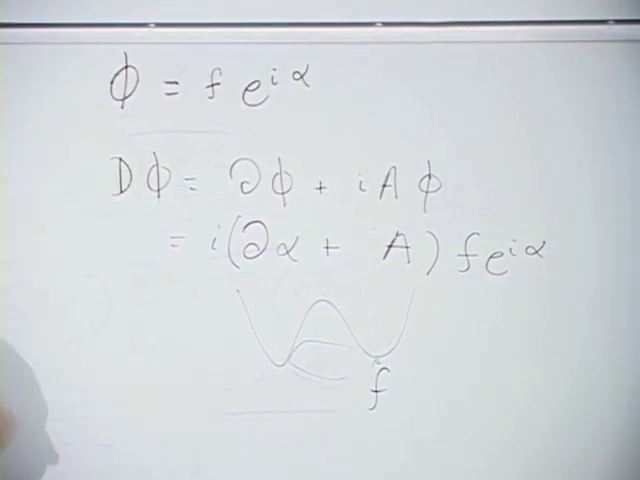
\includegraphics[width=0.72\textwidth]{lecture_09_figure_03.png}
\caption{Der eingefrorene Radius des Higgsfelds, seine kovariante Ableitung und die kleine Skizze des gebrochenen Potentials aus der Wiederholung.}
\lectureframe{00:06:42}
\label{fig:l09-frozen-board}
\end{figure}

Wählen wir die Konvention
\begin{equation}
\begin{aligned}
  D_\mu&=\partial_\mu+igA_\mu,
  \\
  \phi&\longmapsto e^{i\theta}\phi,
  \\
  A_\mu&\longmapsto A_\mu-\frac1g\partial_\mu\theta .
\end{aligned}
  \label{eq:l09-gauge-convention}
\end{equation}
In der Vorlesung wird \(g\) unterdrückt; wenn wir es sichtbar lassen, werden die Dimensionen und die spätere Masse deutlich. Auf das eingefrorene Feld angewandt ergibt sich
\begin{align}
  D_\mu\phi
  &=(\partial_\mu+igA_\mu)f e^{i\alpha}
  \notag\\
  &=i\bigl(\partial_\mu\alpha+gA_\mu\bigr)
    f e^{i\alpha}.
  \label{eq:l09-covariant-frozen}
\end{align}
Die Multiplikation mit der komplex konjugierten Größe beseitigt die Phase und macht außerdem aus \(i\) mal \(-i\) den Faktor \(+1\):
\begin{equation}
  |D_\mu\phi|^2
  =f^2
   \bigl(\partial_\mu\alpha+gA_\mu\bigr)
   \bigl(\partial^\mu\alpha+gA^\mu\bigr).
  \label{eq:l09-frozen-square}
\end{equation}

\begin{classroomqa}
\audiencequestion{Müsste beim Quadrat der kovarianten Ableitung ein Minuszeichen stehen, weil die Ableitung den Faktor \(i\) ergibt?
\lecturetimestamp{00:07:39}}
\lecturerresponse{Nein. Der kinetische Term ist das Produkt mit der komplex konjugierten Größe. Ein Faktor liefert \(i\), der andere \(-i\), und \(i(-i)=1\). Die Vorzeichenkonvention für \(D_\mu\) kann konsistent umgekehrt werden; der Betragsquadratterm ist jedoch im entsprechenden Energieausdruck positiv.}
\end{classroomqa}

Die Kombination in \eqref{eq:l09-frozen-square} ist selbst ein verschobenes Eichfeld. Wählen wir \(\theta=-\alpha\), sodass die Phase des Skalarfelds verschwindet, und definieren wir
\begin{equation}
  A'_\mu=A_\mu+\frac1g\partial_\mu\alpha .
  \label{eq:l09-unitary-gauge-field}
\end{equation}
Dann gilt
\begin{equation}
  |D_\mu\phi|^2=g^2f^2 A'_\mu A'^\mu .
  \label{eq:l09-vector-mass-term}
\end{equation}
Der neue Term enthält keine Ableitung von \(A'_\mu\). Ein homogenes Feld trägt nun Energie, sodass die Vektormode bei verschwindendem Impuls eine Lücke hat.

\begin{figure}[htbp]
\centering
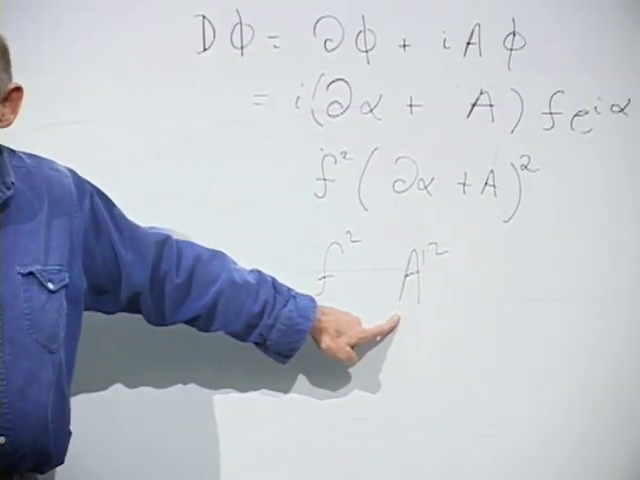
\includegraphics[width=0.72\textwidth]{lecture_09_figure_04.png}
\caption{An der Tafel wird der Term \(f^2A^2\) herausgestellt, der nach Absorption der Phase auf eine Masse des Eichbosons hinweist.}
\lectureframe{00:10:31}
\label{fig:l09-vector-mass-board}
\end{figure}

Bei kanonischer Normierung des Skalarfelds schreibt man
\(\phi=(f+h)e^{i\pi/f}/\sqrt2\). Der Vergleich des resultierenden Vektorterms mit
\(\tfrac12m_A^2A_\mu A^\mu\) ergibt
\begin{equation}
  m_A=gf
  \label{eq:l09-abelian-vector-mass}
\end{equation}
in diesem abelschen Modell. In der Vorlesung werden die Normierungsfaktoren unterdrückt und das Ergebnis mit der Aussage zusammengefasst, dass die Vektormasse durch \(f\) bestimmt wird.

Die Phasenmode ist nicht einfach verschwunden. Vor der Eichung war sie ein masseloses Goldstone-Boson. Nach der Eichung liefert sie die longitudinale Polarisation, die ein massives Vektorteilchen benötigt. Die radiale Fluktuation, die wir vorübergehend eingefroren haben, bleibt als physikalische Higgs-Anregung erhalten.

\subsection{Warum ein Term ohne Ableitungen Masse bedeutet}

\begin{classroomqa}
\audiencequestion{Warum zählt ein Term \(A'^2\) als Masse und nicht einfach als eine weitere Wechselwirkung?\lecturetimestamp{00:13:10}}
\lecturerresponse{Masse ist Ruheenergie. Bei einem Feld ist ein Teilchen in Ruhe das Quant einer Mode mit verschwindendem Impuls und unendlicher Wellenlänge. Der Ableitungsterm liefert einer statischen homogenen Verschiebung keine Energie, \(m_A^2A'^2\) dagegen schon. Diese von null verschiedene Energie bei verschwindendem Impuls ist die Ruheenergielücke.}
\end{classroomqa}

Die Vorlesung erläutert diese Aussage anhand dreier mechanischer Analogien.

\begin{itemize}
  \item In einem Kristall kostet eine langsam variierende Verschiebung elastische Energie, weil benachbarte Atome unterschiedlich verschoben werden. Eine starre Translation verschiebt alle Atome gemeinsam und kostet keine innere Energie. Das akustische Phonon ist daher lückenlos.
  \item In einem idealen rotationssymmetrischen Magneten kostet eine räumlich variierende Spinrichtung Austauschenergie, eine gemeinsame Drehung aller Spins dagegen nicht. Die zugehörige langwellige Spinwelle ist lückenlos.
  \item In einem Plasma erzeugt eine Verschiebung des Elektronenfluids relativ zum positiven Hintergrund eine Ladungstrennung und ein rücktreibendes elektrisches Feld, selbst bei einer homogenen Relativverschiebung. Das daraus entstehende Plasmon hat bei verschwindender Wellenzahl eine von null verschiedene Frequenz.
\end{itemize}

Das mit dem Higgsmechanismus versehene Eichfeld verhält sich wie das dritte Beispiel: Das gebrochene Medium widersetzt sich einer homogenen Verschiebung, die andernfalls keine Energie kosten würde.

\begin{classroomqa}
\audiencequestion{Hat die Phase \(\alpha\) nicht schon vor Einführung des Eichfelds geschwungen?\lecturetimestamp{00:18:24}}
\lecturerresponse{Doch. Ihre Energie war proportional zu \(f^2(\partial_\mu\alpha)^2\). Eine räumlich variierende Phase hat Gradientenenergie und kann sich ausbreiten; eine gleichförmige Phasenänderung kostet jedoch nichts. Genau das ist die masselose Goldstone-Mode.}
\end{classroomqa}

\begin{classroomqa}
\audiencequestion{Die Ableitung enthält auch eine Zeitableitung. Hat die tatsächliche Bewegung des gesamten Gitters oder die Änderung des gesamten Felds dann keine kinetische Energie?\lecturetimestamp{00:22:18}}
\lecturerresponse{Doch. Verglichen werden statische Konfigurationen oder solche, die beliebig langsam vorbereitet werden. Ein Gitter, das sich mit endlicher Geschwindigkeit verschiebt, hat kinetische Energie. Beim Massentest wird gefragt, ob die Konfiguration auch dann Energie hat, wenn sie in Ruhe und räumlich homogen ist.}
\end{classroomqa}

\section{Der experimentelle Hinweis: Die schwache Wechselwirkung unterscheidet links und rechts}

Nun wendet sich die Vorlesung dem Elektron, dem Myon und den Quarks zu. Auch ihre Massen entstehen durch das Higgsfeld, doch der Mechanismus sieht anders aus, weil eine Fermionenmasse kein quadratischer Vektorterm ist. Sie koppelt zwei chirale Felder miteinander.

\subsection{Paritätsverletzung beim Betazerfall}

Ausgangspunkt ist der empirische Befund, dass die schwache Wechselwirkung die Parität verletzt. Die Quantenelektrodynamik und die Quantenchromodynamik behandeln einen Prozess und sein Spiegelbild gleich. Die schwache Wechselwirkung tut das nicht. Beim Betazerfall des Neutrons,
\begin{equation}
  n\longrightarrow p+e^-+\bar\nu_e,
  \label{eq:l09-beta-decay}
\end{equation}
haben die energiereichen Elektronen, die durch die geladene Stromwechselwirkung ausgewählt werden, linkshändige Helizität: Ihr Spin zeigt entgegengesetzt zu ihrem Impuls. Die entsprechenden Antineutrinos haben die entgegengesetzte Helizität.

Für ein ultrarelativistisches Teilchen definieren wir die Helizität durch
\begin{equation}
  h=\frac{\bm S\cdot\bm p}{|\bm S|\,|\bm p|}.
\end{equation}
Spin parallel zum Impuls entspricht \(h=+1\); Spin antiparallel dazu entspricht \(h=-1\). Die schwache Wechselwirkung koppelt an ein linkschirales Elektronenfeld und ein linkschirales Neutrinofeld, nicht in gleicher Weise an ein rechtschirales Elektronenfeld.\editorialnote{Die Vorlesung verwendet zunächst Händigkeit im Sinne der Helizität, weil sie bei hohen Energien anschaulich ist. Eichladungen wirken tatsächlich auf die Chiralität, also auf das Lorentz-Darstellungslabel, das durch \(P_L=(1-\gamma^5)/2\) und \(P_R=(1+\gamma^5)/2\) ausgewählt wird. Bei einem masselosen Teilchen stimmen Chiralität und Helizität für Teilchen überein; bei einem massiven Teilchen ist das nicht der Fall.}

Um das Hindernis ohne die vollständige Buchführung für \(SU(2)_L\times U(1)_Y\) sichtbar zu machen, stellen wir uns eine fiktive Welt mit \(U(1)\) vor, in der nur \(\psi_L\) die betreffende Ladung trägt:
\begin{equation}
  \psi_L\longmapsto e^{i\theta}\psi_L,
  \qquad
  \psi_R\longmapsto\psi_R .
  \label{eq:l09-chiral-toy-charge}
\end{equation}
Das ist nicht Elektromagnetismus: Reale links- und rechtschirale Elektronen tragen dieselbe elektrische Ladung. Es ist eine Karikatur der schwachen Wechselwirkung, bei der die beiden Chiralitäten zu unterschiedlichen elektroschwachen Darstellungen gehören.

\begin{classroomqa}
\audiencequestion{Gilt dieselbe Links--Rechts-Asymmetrie auch für Quarks?
\lecturetimestamp{00:31:50}}
\lecturerresponse{Ja, mit den entsprechenden schwachen Multipletts und Hyperladungen. LinksChirale Up- und Down-Quarks bilden schwache Dubletts, während die rechtschiralen Felder schwache Singuletts sind. Ihre Higgs-Kopplungen stehen deshalb vor demselben strukturellen Problem wie die des Elektrons.}
\end{classroomqa}

\section{Eine Dirac-Masse mischt links--rechts}

\subsection{Von der Vierkomponentengleichung zu zwei Weyl-Gleichungen}

Eine Dirac-Wellenfunktion hat vier Komponenten. Grob gesagt beschreiben zwei davon den Spin, während zwei zwischen Lösungen positiver und negativer Energie unterscheiden; Letztere werden als Freiheitsgrade der Antiteilchen interpretiert. In Hamilton-Form lautet die Gleichung
\begin{equation}
  i\frac{\partial\Psi}{\partial t}
  =\left(-i\bm\alpha\cdot\bm\nabla+m\beta\right)\Psi .
  \label{eq:l09-dirac-hamiltonian}
\end{equation}
Die Matrizen \(\alpha_i\) und \(\beta\) kodieren den relativistischen Zusammenhang zwischen Energie, Impuls und Masse.

\begin{figure}[htbp]
\centering
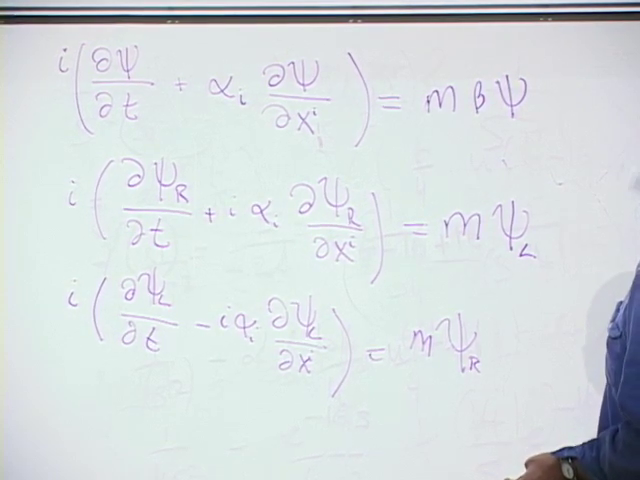
\includegraphics[width=0.74\textwidth]{lecture_09_figure_05.png}
\caption{An der Tafel wird zunächst die Dirac-Gleichung angeschrieben und dann in gekoppelte Gleichungen für links- und rechtshändige Anteile aufgespalten.}
\lectureframe{00:40:30}
\label{fig:l09-dirac-board}
\end{figure}

In der chiralen Basis wird die Rolle von \(m\) deutlich. Mit
\(\sigma^\mu=(1,\bm\sigma)\) und
\(\bar\sigma^\mu=(1,-\bm\sigma)\) gilt
\begin{align}
  i\bar\sigma^\mu\partial_\mu\psi_L&=m\psi_R,
  \label{eq:l09-weyl-left}\\
  i\sigma^\mu\partial_\mu\psi_R&=m\psi_L.
  \label{eq:l09-weyl-right}
\end{align}
Für \(m=0\) sind die Gleichungen unabhängig: Ein links- und ein rechtschirales Feld können sich ausbreiten, ohne miteinander zu wechselwirken. Für \(m\neq0\) tritt jedes der beiden als Quelle des anderen auf. Genau das bedeutet es, dass eine Dirac-Masse links und rechts mischt.

Susskind beschreibt dies als ein Oszillieren des Fermions zwischen links und rechts. Diese Formulierung erfasst die Kopplung, sollte aber nicht als wörtliches klassisches Bild eines Punktteilchens verstanden werden, das hin und her kippt. Die präzise Aussage steckt in der gekoppelten Feldgleichung \eqref{eq:l09-weyl-left}--\eqref{eq:l09-weyl-right}.

\begin{classroomqa}
\audiencequestion{Sind die Faktoren \(i\) und die Vorzeichen in den beiden Gleichungen an der Tafel konsistent?\lecturetimestamp{00:41:10}}
\lecturerresponse{Nicht Zeile für Zeile an der Tafel: Bei der schnellen Herleitung wurde ein \(i\) inkonsistent ausgeklammert. Verlässlich ist das Kopplungsmuster. Die Gleichungen \eqref{eq:l09-weyl-left} und \eqref{eq:l09-weyl-right} entsprechen einer üblichen konsistenten Konvention.}
\end{classroomqa}

\subsection{Warum die schwache Symmetrie eine nackte Masse verbietet}

Der entsprechende Dirac-Massenterm in der Lagrange-Dichte lautet
\begin{equation}
  \mathcal L_m
  =-m\bar\psi\psi
  =-m\left(\bar\psi_L\psi_R+\bar\psi_R\psi_L\right).
  \label{eq:l09-bare-dirac-mass}
\end{equation}
Unter der Spielzeugtransformation \eqref{eq:l09-chiral-toy-charge} gilt
\begin{equation}
  \bar\psi_L\psi_R\longmapsto
  e^{-i\theta}\bar\psi_L\psi_R,
  \qquad
  \bar\psi_R\psi_L\longmapsto
  e^{i\theta}\bar\psi_R\psi_L.
\end{equation}
Keiner der beiden Terme ist invariant. Der direkte Koeffizient \(m\) für die Links--Rechts-Mischung ist daher vor der Symmetriebrechung verboten.

Der Elektromagnetismus allein würde dieses Problem nicht verursachen, denn \(\psi_L\) und \(\psi_R\) haben dieselbe elektrische Ladung. Das Hindernis entsteht durch ihre unterschiedlichen schwachen Quantenzahlen.

\subsection{Helizitätsfragen, die die Feinheiten der Chiralität sichtbar machen}

Nun prüft der Kurs das anschauliche Bild der Händigkeit aus mehreren Blickwinkeln. Diese Fragen sind keine Nebensache: Sie zeigen genau, wo die Helizität hilfreich ist und wo man stattdessen die Chiralität heranziehen muss.

\begin{classroomqa}
\audiencequestion{Wie sähe die Welt aus, wenn die schwache Wechselwirkung Elektronen mit beiden Helizitäten gleich häufig emittierte?\lecturetimestamp{00:42:12}}
\lecturerresponse{Die unmittelbare Paritätsasymmetrie in diesem Prozess wäre dann nicht vorhanden. Die reale elektroschwache Theorie ist jedoch chiral: Nur die linkschiralen Dubletts tragen die geladene schwache Wechselwirkung. Die Vorlesung verschiebt eine ausführlichere Erklärung dafür, warum die Natur diese Struktur gewählt hat, auf später.}
\end{classroomqa}

\begin{classroomqa}
\audiencequestion{Angenommen, der Spin eines Elektrons wird vertikal präpariert und das Elektron anschließend horizontal beschleunigt. Ist es links- oder rechtshändig?
\lecturetimestamp{00:42:44}}
\lecturerresponse{Ein Spin-Zustand, der quer zum Impuls steht, ist eine Überlagerung der beiden Helizitäten. Eine scharfe Helizität liegt nur vor, wenn der Spin parallel oder antiparallel zum Impuls ist. Die chiralen Projektoren der schwachen Wechselwirkung sind für das Feld dennoch wohldefiniert.}
\end{classroomqa}

Ein massives Teilchen kann bis zum Stillstand abgebremst und in die entgegengesetzte Richtung beschleunigt werden, ohne seinen Spin umzudrehen. Dabei ändert seine Helizität das Vorzeichen. Ein masseloses Teilchen kann durch einen Lorentz-Boost weder überholt noch zum Stillstand gebracht werden; seine Helizität bleibt daher unter eigentlichen Boosts invariant. Das motiviert die Aussage der Vorlesung, dass eine Teilchensorte mit nur einer physikalischen Helizität masselos sein muss. Präziser lautet die feldtheoretische Aussage: Eine Lorentz-invariante Dirac-Masse erfordert beide Chiralitäten.

\begin{classroomqa}
\audiencequestion{Ein zirkular polarisiertes Photon kann an einem Spiegel reflektiert werden und seine Ausbreitungsrichtung umkehren, ohne jemals zum Stillstand zu kommen. Widerspricht das dem Helizitätsargument?
\lecturetimestamp{00:45:28}}
\lecturerresponse{Nein. Der Spiegel ist ein äußeres System, das Drehimpuls austauschen und die Ausbreitungsrichtung umkehren kann. Eine Reflexion ist kein Lorentz-Boost, der das Photon überholt. Ob ein Kanal existiert, hängt außerdem von den erlaubten Polarisationszuständen und den Randbedingungen des Materials ab.}
\end{classroomqa}

\begin{classroomqa}
\audiencequestion{Enthält ein gewöhnlicher Elektronenstrahl eine oder beide Händigkeiten?
\lecturetimestamp{00:46:10}}
\lecturerresponse{Im Allgemeinen beide. Ein Zustand eines massiven Elektrons enthält beide chiralen Komponenten, und ein unpolarisierter Strahl enthält beide Helizitäten. Spezielle Quellen können einen polarisierten Strahl mit einer starken Helizitätsasymmetrie erzeugen.}
\end{classroomqa}

\begin{classroomqa}
\audiencequestion{Kann ein Strahl unabhängig vom Spin fokussiert werden, oder trennen Magnetfelder die beiden Polarisationen?
\lecturetimestamp{00:46:29}}
\lecturerresponse{Eine gewöhnliche Ortsfokussierung kann weitgehend spinunabhängig sein, doch magnetische Momente koppeln an Gradienten des Magnetfelds. Spinselektive Quellen, Stern--Gerlach-artige Gradienten und die Spindynamik im Beschleuniger können daher Polarisationen präparieren oder voneinander trennen.}
\end{classroomqa}

\begin{classroomqa}
\audiencequestion{Ist der Unterschied zwischen links und rechts bei der schwachen Wechselwirkung bloß Zufall?
\lecturetimestamp{00:48:13}}
\lecturerresponse{Im Rahmen dieses Kurses ist er ein experimenteller Befund, der im Standardmodell verankert ist. Er ist so systematisch, dass er kaum wie ein beiläufiger Zufall wirkt; doch das Standardmodell selbst leitet das vollständige Muster der chiralen Ladungen nicht aus einem tieferen Prinzip her.}
\end{classroomqa}

\section{Die Yukawa-Konstruktion}

\subsection{Das Higgsfeld die fehlende Ladung tragen lassen}

Die Symmetrie verbietet eine numerische Masse, erlaubt aber eine Wechselwirkung mit einem Feld, das die fehlende Transformationsphase beisteuert. Führen wir ein komplexes Skalarfeld ein mit
\begin{equation}
  \phi\longmapsto e^{i\theta}\phi,
  \qquad
  \phi^\dagger\longmapsto e^{-i\theta}\phi^\dagger.
  \label{eq:l09-scalar-charge}
\end{equation}
Dann ist
\begin{equation}
  \mathcal L_Y
  =-y\,\bar\psi_L\phi\psi_R
   -y^*\,\bar\psi_R\phi^\dagger\psi_L
  \label{eq:l09-yukawa-lagrangian}
\end{equation}
eichinvariant. Im ersten Term trägt \(\bar\psi_L\) den Faktor \(e^{-i\theta}\) bei und \(\phi\) den Faktor \(e^{i\theta}\); die Phasen heben sich auf. Der zweite Term ist die hermitesch konjugierte Größe.

Entsprechend erhalten die chiralen Gleichungen eine feldabhängige Mischung:
\begin{align}
  i\bar\sigma^\mu D_\mu\psi_L
    &=y\phi\psi_R,
  \label{eq:l09-yukawa-eom-left}\\
  i\sigma^\mu\partial_\mu\psi_R
    &=y^*\phi^\dagger\psi_L.
  \label{eq:l09-yukawa-eom-right}
\end{align}

\begin{figure}[htbp]
\centering
\includegraphics[width=0.76\textwidth]{lecture_09_figure_06.png}
\caption{Die nackte Masse auf den rechten Seiten wurde durch das geladene Skalarfeld ersetzt. Die genauen Vorzeichen an der Tafel sind schematisch; die invariante Struktur steht in \eqref{eq:l09-yukawa-lagrangian}.}
\lectureframe{00:51:30}
\label{fig:l09-yukawa-board}
\end{figure}

Vor der Symmetriebrechung handelt es sich hierbei um eine Wechselwirkung und nicht um eine Masse. Ein rechtschirales Fermion kann nur dann in ein linkschirales Fermion übergehen, wenn es das Skalarquant emittiert oder absorbiert, das zum Ausgleich der Ladung erforderlich ist. Der Koeffizient \(y\) ist eine Yukawa-Kopplung und nicht die Eichladung \(g\).

\begin{classroomqa}
\audiencequestion{Ist es zulässig, einfach \(\phi\) und \(\phi^\dagger\) auf die rechten Seiten der beiden Gleichungen zu setzen?
\lecturetimestamp{00:51:55}}
\lecturerresponse{Das ist genau deshalb zulässig, weil ihre Transformationsphasen die Abweichung ausgleichen. Entscheidend ist nicht die äußere Form der Gleichung, sondern die Eichinvarianz der Wechselwirkung \(\bar\psi_L\phi\psi_R+\mathrm{h.c.}\).}
\end{classroomqa}

\subsection{Das Vakuum macht aus der Wechselwirkung eine Masse}

Identifizieren wir nun \(\phi\) mit dem Higgsfeld und lassen es einen von null verschiedenen Vakuumbetrag annehmen. In der vereinfachten Normierung der Vorlesung gilt
\begin{equation}
  \phi\simeq f,
\end{equation}
sodass \eqref{eq:l09-yukawa-lagrangian} den Term
\begin{equation}
  \mathcal L_Y
  \supset
  -yf\,\bar\psi_L\psi_R
  -y^*f\,\bar\psi_R\psi_L .
\end{equation}enthält. Nach einer unproblematischen Phasenumdefinition, sofern nötig, ist die Fermionenmasse
\begin{equation}
  m_f=yf.
  \label{eq:l09-lecture-fermion-mass}
\end{equation}
Dies ist das fermionische Gegenstück zum Vektorergebnis \(m_A=gf\). Dasselbe Higgs-Vakuum, das den schwachen Eichbosonen eine longitudinale Polarisation verleiht, liefert auch die fehlenden schwachen Quantenzahlen, die nötig sind, um links- und rechtschirale Fermionen zu verbinden.

In der kanonisch normierten Konvention des Standardmodells gilt
\begin{equation}
  H(x)=\frac1{\sqrt2}
  \begin{pmatrix}
    0\\ v+h(x)
  \end{pmatrix},
  \qquad v\simeq246\ \mathrm{GeV},
  \label{eq:l09-sm-higgs-vacuum}
\end{equation}
und damit
\begin{equation}
  m_f=\frac{y_fv}{\sqrt2}.
  \label{eq:l09-sm-fermion-mass}
\end{equation}
Das \(f\) der Vorlesung und die übliche Größe \(v/\sqrt2\) unterscheiden sich lediglich aufgrund dieser Normierungswahl.

\begin{classroomqa}
\audiencequestion{Wenn nur das Produkt \(yf\) eine Fermionenmasse ist, wie lassen sich die Kopplung \(y\) und die Vakuumskala \(f\) getrennt bestimmen?
\lecturetimestamp{00:55:36}}
\lecturerresponse{Sobald die Eichkopplungen bekannt sind, legen die Massen der schwachen Eichbosonen die Vakuumskala fest. Aus der gemessenen Masse eines Fermions ergibt sich dann dessen Yukawa-Kopplung. In der vollständigen Theorie gilt \(m_W=gv/2\), \(m_Z=v\sqrt{g^2+g'^2}/2\) und \(y_f=\sqrt2m_f/v\).}
\end{classroomqa}

\begin{classroomqa}
\audiencequestion{Liegt die Masse des schwachen Eichbosons bei etwa \(900\ \mathrm{GeV}\)?
\lecturetimestamp{00:57:43}}
\lecturerresponse{Nein; die Vorlesung korrigiert den Versprecher unmittelbar auf ungefähr \(90\ \mathrm{GeV}\). Genauer gilt \(m_W\simeq80\ \mathrm{GeV}\) und \(m_Z\simeq91\ \mathrm{GeV}\), während die zugrunde liegende Vakuumskala \(v\simeq246\ \mathrm{GeV}\) beträgt.}
\end{classroomqa}

\subsection{Eine Vakuumskala, viele Yukawa-Kopplungen}

Jede geladene Fermionensorte hat ihre eigene Yukawa-Kopplung:
\begin{equation}
  m_i=y_i f
  \qquad\text{(lecture normalization)}.
  \label{eq:l09-mass-family}
\end{equation}

\begin{figure}[htbp]
\centering
\includegraphics[width=0.76\textwidth]{lecture_09_figure_08.png}
\caption{An der Tafel wird die Abhängigkeit von der Teilchensorte als \(m_i=g_i f\) zusammengefasst; die dort notierten \(g_i\) sind die Yukawa-Kopplungen, die hier \(y_i\) heißen.}
\lectureframe{01:16:30}
\label{fig:l09-mass-family-board}
\end{figure}

Für das Elektron schätzt die Vorlesung
\begin{equation}
  y_e\sim\frac{0.5\ \mathrm{MeV}}{10^2\ \mathrm{GeV}}
  \sim10^{-5}.
\end{equation}
Mit dem kanonischen Wert \(v=246\ \mathrm{GeV}\) ergibt sich genauer
\(y_e\simeq2.9\times10^{-6}\). Das Top-Quark liegt am entgegengesetzten Ende:
\begin{equation}
  y_t=\frac{\sqrt2m_t}{v}\simeq1.
\end{equation}
Der Higgs-Mechanismus erklärt also, wie eine eichinvariante Masse existieren kann, nicht aber die enorme Hierarchie zwischen den \(y_i\). Die beobachteten Fermionenmassen bringen diese Hierarchie lediglich in Form messbarer Zahlen zum Ausdruck.

\begin{classroomqa}
\audiencequestion{Hat das Top-Quark tatsächlich eine Yukawa-Kopplung von der Größenordnung eins?
\lecturetimestamp{00:59:09}}
\lecturerresponse{Ja. Seine Masse ist mit der elektroschwachen Skala vergleichbar, daher ist seine Kopplung keine winzige Störungsgröße wie die des Elektrons. In der modernen Normierung liegt \(y_t\) nahe bei eins.}
\end{classroomqa}

\subsection{Die physikalische Higgs-Fluktuation wieder einsetzen}

Das Einfrieren des Skalarfelds auf seinen Vakuumwert hat die radiale Anregung verborgen. Setzen wir sie schematisch wieder ein:
\begin{equation}
  \phi(x)\simeq f+h(x).
\end{equation}
Der Yukawa-Faktor wird dann zu
\begin{equation}
  y\phi\simeq yf+yh=m_f+yh.
  \label{eq:l09-mass-plus-higgs}
\end{equation}

\begin{figure}[htbp]
\centering
\includegraphics[width=0.76\textwidth]{lecture_09_figure_07.png}
\caption{An der Tafel wird die Higgs-Fluktuation wieder in den Yukawa-Term eingesetzt: Der konstante Anteil erzeugt die Fermionenmasse, der fluktuierende Anteil die Emission oder Absorption von Higgs-Bosonen.}
\lectureframe{01:01:15}
\label{fig:l09-higgs-fluctuation-board}
\end{figure}

Der erste Term in \eqref{eq:l09-mass-plus-higgs} ist die Masse. Der zweite ist ein Vertex, an dem ein Higgs-Boson an das Fermion koppelt. In der kanonischen Notation des Standardmodells gilt
\begin{equation}
  \mathcal L_Y
  \supset
  -m_f\bar\psi\psi
  -\frac{m_f}{v}h\bar\psi\psi.
  \label{eq:l09-higgs-fermion-vertex}
\end{equation}
Die Kopplung ist proportional zur Fermionenmasse. Unter Berücksichtigung der Kinematik, der Farbzahl, des Phasenraums und konkurrierender Kanäle koppelt das Higgs-Boson daher stärker an schwerere Fermionen.

\begin{classroomqa}
\audiencequestion{Sind Kopplungskonstanten selbst Wahrscheinlichkeiten?
\lecturetimestamp{01:03:35}}
\lecturerresponse{Sie gehen in quantenmechanische Amplituden ein. Eine einfache Rate ist oft proportional zum Betragsquadrat einer Amplitude und damit zum Quadrat einer Kopplung; außerdem spielen aber Phasenraum, Spinsummen, Interferenz, Schleifen und mehrere Vertizes eine Rolle. Eine Kopplung sollte nicht unmittelbar mit einer Wahrscheinlichkeit gleichgesetzt werden.}
\end{classroomqa}

\begin{classroomqa}
\audiencequestion{Setzt diese Argumentation voraus, dass es nur ein Higgsfeld gibt?
\lecturetimestamp{01:03:59}}
\lecturerresponse{Sie beschreibt das minimale Standardmodell mit einem komplexen Higgs-Dublett. Drei seiner vier reellen Komponenten werden von \(W^\pm\) und \(Z\) absorbiert; übrig bleibt ein physikalisches neutrales Skalarteilchen. Erweiterungen können weitere Dubletts oder andere Skalarmultipletts enthalten. Supersymmetrische Modelle benötigen typischerweise zwei Higgs-Dubletts und enthalten deshalb mehrere physikalische Higgs-Zustände.}
\end{classroomqa}

Diese historische Erwartung lässt sich nun mit dem Experiment vergleichen.
\editorialnote{Diese Vorlesung wurde vor der Entdeckung des Higgs-Bosons aufgezeichnet. ATLAS und CMS gaben 2012 die Entdeckung eines Higgs-ähnlichen Teilchens bekannt, dessen Masse inzwischen mit etwa \(125\ \mathrm{GeV}\) gemessen wird. Seine beobachteten Kopplungen stimmen im Großen und Ganzen mit dem massenproportionalen Muster des Standardmodells überein. Die Aussage, dass es bevorzugt in die schwersten Teilchen zerfällt, gilt stets mit einer kinematischen Einschränkung: Ein on-shell erzeugtes \(t\bar t\)-Paar ist für ein Higgs-Boson mit einer Masse von \(125\ \mathrm{GeV}\) zu schwer.}

\section{Antiteilchen, Strahlen und die Bedeutung der Chiralität}

Bevor sich der Kurs den Neutrinos zuwendet, kehrt er zu einigen praktischen Fragen über Antiteilchen und Teilchenstrahlen zurück.

\begin{classroomqa}
\audiencequestion{Welche Händigkeit hat das Antiteilchen eines linkshändigen Elektrons?
\lecturetimestamp{01:06:05}}
\lecturerresponse{Ein linkschirales Elektronenfeld vernichtet Elektronen mit linkshändiger Helizität und erzeugt im ultrarelativistischen Grenzfall Positronen mit rechtshändiger Helizität. Hier müssen Teilchen und Antiteilchen sowie Chiralität und Helizität besonders sorgfältig auseinandergehalten werden.}
\end{classroomqa}

\begin{classroomqa}
\audiencequestion{Können ein Elektron und ein Positron zu einem \(Z\)-Boson kollidieren?
\lecturetimestamp{01:07:13}}
\lecturerresponse{Ja, wenn ihre Schwerpunktsenergie dem erlaubten Kanal entspricht. Elektron--Positron-Collider haben die \(Z\)-Resonanz mit großer Präzision untersucht. Ladung und die übrigen Quantenzahlen bleiben im Gesamtprozess erhalten.}
\end{classroomqa}

\begin{classroomqa}
\audiencequestion{Entstehen Positronen alle durch einen einzigen besonderen schwachen Prozess?
\lecturetimestamp{01:07:37}}
\lecturerresponse{Nein. Paarerzeugung ist ein gewöhnlicher elektromagnetischer Prozess. Zum Beispiel kann ein energiereiches Elektron ein virtuelles Photon abstrahlen, und dieses Photon kann im Feld eines anderen Teilchens ein \(e^-e^+\)-Paar erzeugen. Die Vorlesung skizziert dies mit einem Feynman-Diagramm.}
\end{classroomqa}

\begin{classroomqa}
\audiencequestion{Kann ein Linearbeschleuniger die Geschwindigkeit oder Energie seiner Elektronen auswählen?
\lecturetimestamp{01:09:24}}
\lecturerresponse{Ja. Die Beschleunigungsfelder und die zeitliche Abstimmung legen einen Energiebereich fest. Sobald die Elektronen ultrarelativistisch sind, ist ihre Geschwindigkeit bereits extrem nahe an \(c\); zusätzliche Beschleunigerenergie erhöht daher vor allem Impuls und Gesamtenergie, statt die Geschwindigkeit sichtbar zu steigern.}
\end{classroomqa}

\begin{classroomqa}
\audiencequestion{Kann ein Beschleuniger einen Strahl mit einer einzigen Polarisation präparieren?
\lecturetimestamp{01:09:47}}
\lecturerresponse{Ja, auch wenn das technisch anspruchsvoll ist. Bei niedriger Energie lassen sich mit einer spinabhängigen Quelle spinpolarisierte Elektronen erzeugen und anschließend beschleunigen, während man die Spinpräzession kontrolliert. Moderne Collider quantifizieren die resultierende Strahlpolarisation, statt sie als vollkommen rein zu behandeln.}
\end{classroomqa}

\section{Neutrinomasse und die Majorana-Möglichkeit}

\subsection{Warum Neutrinomassen eine Erweiterung erforderten}

Das ursprüngliche minimale Standardmodell enthielt nur linkschirale Neutrinofelder und sagte daher masselose Neutrinos voraus. Neutrinooszillationen zeigen, dass sich mindestens zwei Neutrinomasseneigenwerte unterscheiden und Neutrinos somit eine von null verschiedene Masse haben, auch wenn diese im Vergleich zu den Massen geladener Fermionen winzig ist.

\begin{classroomqa}
\audiencequestion{Wie klein sind die Neutrinomassen, und wo ist ihre rechtschirale Komponente?
\lecturetimestamp{01:10:38}}
\lecturerresponse{Oszillationen bestimmen Massendifferenzen zum Quadrat, nicht die absoluten Massen. Die relevanten Massendifferenzen entsprechen ungefähr den Skalen \(0.009\ \mathrm{eV}\) und \(0.05\ \mathrm{eV}\). Eine Dirac-Beschreibung führt sterile rechtschirale Neutrinos ein; eine Majorana-Beschreibung setzt die fehlende Chiralität stattdessen mit ladungskonjugierten Neutrinofeldern in Beziehung.}
\end{classroomqa}

Für ein Dirac-Neutrino fügt man ein neues Feld \(\nu_R\) hinzu und wiederholt die Yukawa-Konstruktion:
\begin{equation}
  \mathcal L_{\nu,\mathrm{Dirac}}
  =-y_\nu\bar L\,\widetilde H\,\nu_R+\mathrm{h.c.},
  \qquad
  m_\nu=\frac{y_\nu v}{\sqrt2}.
  \label{eq:l09-dirac-neutrino}
\end{equation}
Das erforderliche \(y_\nu\) ist außerordentlich klein.

Es gibt noch eine weitere logische Möglichkeit, denn das Neutrino trägt keine elektrische Ladung. Ein linkschirales Neutrino kann an sein eigenes ladungskonjugiertes Feld gekoppelt werden, das die entgegengesetzte Chiralität besitzt:
\begin{equation}
  \nu_L\longleftrightarrow(\nu_L)^c_R .
  \label{eq:l09-majorana-mixing}
\end{equation}
Ein so gebildeter Masseneigenzustand ist ein Majorana-Fermion: Bis auf Phasenkonventionen ist es sein eigenes Antiteilchen. Eine analoge Elektron--Positron-Mischung ist verboten, weil sie die exakte Erhaltung der elektrischen Ladung verletzen würde.

\begin{classroomqa}
\audiencequestion{Warum ist eine Teilchen--Antiteilchen-Mischung bei einem Neutrino erlaubt, bei einem Elektron aber nicht?\lecturetimestamp{01:13:43}}
\lecturerresponse{Elektron und Positron haben entgegengesetzte elektrische Ladungen. Ein Massenterm, der sie als denselben Einteilchenzustand mischt, würde daher die ungebrochene elektromagnetische Symmetrie verletzen. Ein Neutrino ist elektrisch neutral. Wenn keine exakt erhaltene Leptonenzahl es von seinem Antiteilchen unterscheidet, ist eine Majorana-Masse erlaubt.}
\end{classroomqa}

Der Name ehrt Ettore Majorana, den jungen italienischen Physiker, der diese Art reeller Fermionendarstellung formulierte und 1938 verschwand. Die Vorlesung hält bei diesem historischen Rätsel inne: Sein Schicksal wurde nie aufgeklärt.
\editorialnote{Eine eichinvariante Majorana-Masse für das aktive Neutrino des Standardmodells ist vor der elektroschwachen Symmetriebrechung kein renormierbarer nackter Term. Bei niedrigen Energien kann sie aus dem Weinberg-Operator der Dimension fünf \((LH)(LH)/\Lambda\) oder über einen Seesaw-Mechanismus mit schweren sterilen Neutrinos entstehen. Ob Neutrinos Dirac- oder Majorana-Teilchen sind, ist experimentell weiterhin ungeklärt.}

\section{Warum sich das vertraute Spektrum nahe der elektroschwachen Skala häuft}

\subsection{Die gemeinsame Skala und ihre wichtigen Einschränkungen}

\begin{classroomqa}
\audiencequestion{Warum erwartete man, dass die Higgs-Masse im Bereich der schwachen Skala liegen würde?\lecturetimestamp{01:14:48}}
\lecturerresponse{Die Krümmung des Higgs-Potentials legt die radiale Higgs-Masse fest, während dieselbe Vakuumskala \(f\) die Massen von \(W\) und \(Z\) bestimmt. Ohne eine extrem große skalare Selbstkopplung erwartete man daher, dass die Higgs-Masse größenordnungsmäßig in der Nähe der schwachen Skala liegt. Der beobachtete Wert \(125\ \mathrm{GeV}\) liegt tatsächlich in diesem Bereich.}
\end{classroomqa}

Die prägnante Zusammenfassung der Vorlesung lautet: Die Elementarmassen des minimalen Standardmodells gehen auf ein einziges gebrochenes Vakuum zurück:
\begin{align}
  m_W&=\frac12gv,\\
  m_Z&=\frac12\sqrt{g^2+g'^2}\,v,\\
  m_f&=\frac1{\sqrt2}y_fv.
  \label{eq:l09-electroweak-mass-summary}
\end{align}
Wenn \(v\) verschwände, während die dimensionslosen Kopplungen unverändert blieben, wären die schwachen Eichbosonen und die geladenen Elementarfermionen masselos.

Diese Aussage darf nicht über ihren Gültigkeitsbereich hinaus verallgemeinert werden. Photon und Gluonen bleiben masselos, weil eine ungebrochene Eichsymmetrie sie schützt. Der größte Teil der Protonen- und Neutronenmasse ist QCD-Bindungsenergie und nicht die Summe der Higgs-Massen ihrer Quarks. Neutrinomassen erfordern eine Erweiterung des minimalen Modells. Die Higgs-Masse selbst hängt vom skalaren Potential ab und ist nicht einfach eine weitere Yukawa-Masse.

\subsection{Teilchen, deren Masse nicht auf die Symmetriebrechung warten muss}

Angenommen, ein neues Fermion hätte links- und rechtsschirale Komponenten mit denselben Eichquantenzahlen. Dann wäre \(\bar\Psi_L\Psi_R+\mathrm{h.c.}\) bereits eichinvariant. Ein solches \emph{vektorartiges} Fermion könnte eine nackte Masse \(M\) besitzen, die unabhängig von \(v\) ist:
\begin{equation}
  \mathcal L_{\mathrm{vectorlike}}
  =-M\bar\Psi\Psi.
  \label{eq:l09-vectorlike-mass}
\end{equation}
Für \(M\gg v\) gibt es kein elektroschwaches Symmetriehindernis.

Das motiviert das weit gefasste Natürlichkeitsargument der Vorlesung. Teilchen, die durch Eich- oder chirale Symmetrie geschützt sind, bleiben masselos, bis das Higgs-Vakuum diesen Schutz aufhebt; ihre Massen sind daher an die vergleichsweise kleine Skala \(v\) gebunden. Teilchen ohne einen solchen Schutz können natürlicherweise viel schwerer sein und deshalb im beobachteten Niederenergiespektrum fehlen. Was wir sehen, könnte ein Selektionseffekt sein: Die zugänglichen Teilchen sind diejenigen, deren Massen durch die elektroschwache Symmetriebrechung bedingt erst entstehen konnten.

\begin{classroomqa}
\audiencequestion{Würden Teilchen mit unabhängig davon viel größeren Massen in der Wirklichkeit keine Rolle spielen?\lecturetimestamp{01:19:39}}
\lecturerresponse{In der gewöhnlichen Niederenergie-Laborphysik würden sie nur eine geringe Rolle spielen, weil sie schwer zu erzeugen sind. Die Geschichte des Universums bei hohen Energien oder die Kosmologie könnten sie dennoch beeinflussen. Die Vorlesung nennt dunkle Materie als möglichen Bereich, in dem sich ein schwereres verborgenes Spektrum zuerst bemerkbar machen könnte.}
\end{classroomqa}

Die Diskussion von 2010 spiegelt die damals verbreitete Erwartung dunkler Materie im Bereich der schwachen Skala oder etwas darüber wider. Das ist weiterhin eine nützliche Modellklasse, aber keine gesicherte Tatsache. Dunkle Materie wurde durch ihre Gravitation nachgewiesen; ihre Teilchennatur und der Ursprung ihrer Masse sind jedoch unbekannt.

\section{Abschließende Fragen: kosmische Strahlung, Trägheit, Gravitation und Chiralität}

\subsection{Masse ist keine hohe Laborenergie}

\begin{classroomqa}
\audiencequestion{Welche Masse hat ein Teilchen der kosmischen Strahlung?
\lecturetimestamp{01:20:57}}
\lecturerresponse{Ein Teilchen der kosmischen Strahlung kann ein Proton, ein Atomkern, ein Elektron oder ein Photon sein; seine invariante Masse ist die Masse dieses Teilchens oder Systems. Bemerkenswert ist seine Laborenergie, die bei den energiereichsten Ereignissen ungefähr \(10^{20}\) bis \(10^{21}\ \mathrm{eV}\) erreicht. Hohe Energie ist nicht dasselbe wie hohe invariante Masse.}
\end{classroomqa}

Ein Teilchen der kosmischen Strahlung trifft auf ein Zielteilchen, das sich näherungsweise in Ruhe befindet. Für ein Projektilproton mit der Laborenergie \(E\gg m_p\) gilt:
\begin{equation}
  s=(p_1+p_2)^2
  \simeq2m_pE+2m_p^2,
  \qquad
  \sqrt{s}\simeq\sqrt{2m_pE}.
  \label{eq:l09-fixed-target-s}
\end{equation}
Nur die Quadratwurzel der Projektilenergie wird zur Schwerpunktsenergie. Für zwei gleiche, frontal aufeinanderprallende Strahlen mit der Energie \(E_{\rm beam}\) gilt:
\begin{equation}
  \sqrt{s}\simeq2E_{\rm beam}.
  \label{eq:l09-collider-s}
\end{equation}
Deshalb wandelt ein Collider kontrollierte Strahlenergie viel effizienter in die Masse neuer Teilchen um als ein Experiment mit ruhendem Target.

\begin{classroomqa}
\audiencequestion{Warum kann der Collider am CERN ein leistungsfähigeres Werkzeug sein als ein einzelnes, viel energiereicheres Teilchen, das auf ruhende Materie trifft?
\lecturetimestamp{01:21:50}}
\lecturerresponse{Bei einer Kollision an einem ruhenden Target trägt die Impulserhaltung dazu bei, dass der größte Teil der Laborenergie in der Bewegung des Endzustands weitergetragen wird. Bei einem symmetrischen Collider kann der gesamte räumliche Impuls verschwinden, sodass die Strahlenergie als Schwerpunktsenergie zur Verfügung steht. Die energiereichsten kosmischen Strahlungsteilchen können den LHC bei \(\sqrt{s}\) zwar übertreffen, treffen aber unvorhersehbar ein und ermöglichen weder die Luminosität eines Colliders noch eine kontrollierte Detektorumgebung.}
\end{classroomqa}

\subsection{Ruhemasse und Widerstand gegen Beschleunigung}

\begin{classroomqa}
\audiencequestion{Sind Trägheit und Masse im Wesentlichen dasselbe?
\lecturetimestamp{01:22:41}}
\lecturerresponse{In Ruhe ist die invariante Masse sowohl über \(E_0=mc^2\) mit der Ruheenergie verknüpft als auch der Parameter, der die Reaktion auf eine Kraft bei niedrigen Geschwindigkeiten bestimmt. Die spezielle Relativitätstheorie erklärt, warum diese beiden Definitionen zu derselben Größe gehören. Bei bewegten Körpern ist es klarer, die invariante Masse konstant zu halten und die Beschleunigung mithilfe relativistischer Energie und relativistischem Impuls zu beschreiben.}
\end{classroomqa}

Die invariante Beziehung
\begin{equation}
  E^2=p^2c^2+m^2c^4
  \label{eq:l09-energy-momentum}
\end{equation}
enthält beide Bedeutungen. In der Nähe des Ruhezustands gilt
\begin{equation}
  E=mc^2+\frac{p^2}{2m}+\cdots,
\end{equation}
sodass dieselbe Masse \(m\), die die Ruheenergie bestimmt, auch in der kinetischen Reaktion auftritt. Bei hohen Geschwindigkeiten hängt der Zusammenhang zwischen Kraft und Beschleunigung davon ab, ob die Kraft parallel oder senkrecht zur Geschwindigkeit wirkt. Wegen dieser Richtungsabhängigkeit vermeidet man in modernen Darstellungen die geschwindigkeitsabhängige \emph{relativistische Masse} und bezeichnet nur die Lorentz-invariante Größe \(m\) als Masse.

\subsection{Woran die Gravitation koppelt}

\begin{classroomqa}
\audiencequestion{Koppelt ein Teilchen, sobald das Higgs ihm Masse verleiht, auch an die Gravitation?\lecturetimestamp{01:23:58}}
\lecturerresponse{Seine Ruheenergie trägt zur Gravitation bei, aber die Masse ist nicht die ganze Quelle. Photonen sind masselos und werden dennoch durch die Gravitation abgelenkt. In der allgemeinen Relativitätstheorie ist der Energie--Impuls-Tensor die Quelle: Energiedichte, Impulsstrom, Druck und Spannung. Bei langsam bewegter Materie ist der Beitrag ihrer Ruhemasseenergie dominant.}
\end{classroomqa}

Die Ablenkung des Lichts nahe der Sonne macht dies anschaulich. Ein Photon reagiert auf die Raumzeitkrümmung, obwohl es \(m=0\) hat; auch seine Energie und sein Impuls tragen zum Gravitationsfeld bei. Bei zwei nahezu ruhenden massiven Körpern wird die Energie von \(mc^2\) dominiert, sodass sich die Newtonsche Gravitation durch ihre Massen ausdrücken lässt, ohne die allgemeinere Aussage zum Energie--Impuls-Tensor hinzuschreiben.

\begin{classroomqa}
\audiencequestion{Lässt sich ein hochenergetisches Teilchen in jeder Richtung gleich schwerer beschleunigen?\lecturetimestamp{01:25:20}}
\lecturerresponse{Nein. Die Impulsänderung bei einer Kraft parallel zur Bewegung unterscheidet sich von der bei einer transversalen Kraft. Es stimmt, dass ein energiereicheres Teilchen schwerer abzulenken ist; ihm eine einzige vergrößerte Bewegungsmasse zuzuschreiben, verschleiert jedoch diese Richtungsabhängigkeit.}
\end{classroomqa}

\subsection{Ein ruhendes Elektron und die angekündigte Unterscheidung}

\begin{classroomqa}
\audiencequestion{Wie kann man ein ruhendes Elektron als links- oder rechtshändig bezeichnen?\lecturetimestamp{01:26:32}}
\lecturerresponse{Das geht nicht über seine Helizität, denn diese ist über die Impulsrichtung definiert. Ein Ruhespinor lässt sich dennoch in links- und rechtsschirale Komponenten zerlegen. Bei einem massiven Elektron sind beide Komponenten vorhanden, und der Massenterm koppelt sie.}
\end{classroomqa}

\begin{classroomqa}
\audiencequestion{Kann ein ruhendes Elektron an einer schwachen Wechselwirkung teilnehmen, obwohl es keine Helizität hat?\lecturetimestamp{01:27:18}}
\lecturerresponse{Ja. Die schwache Wechselwirkung koppelt an die Chiralität, nicht an eine bezugssystemabhängige Helizität. Bei hohen Energien ist die Helizität eine zweckmäßige Näherung für die Chiralität; in der Nähe des Ruhezustands versagt diese Näherung. Das ist die subtile Unterscheidung, die die Vorlesung bis hierhin aufgeschoben hatte.}
\end{classroomqa}

\section{Historische Fragen zum Ende der Vorlesung}

\subsection{Das Higgs-Massenfenster vor seiner Entdeckung}

Im Jahr 2010 war das Higgs noch nicht entdeckt. Präzisionsmessgrößen der elektroschwachen Wechselwirkung, insbesondere schleifensensitive Beziehungen zwischen \(W\), \(Z\), dem Top-Quark und weiteren Parametern, sprachen innerhalb des Standardmodells für ein vergleichsweise leichtes Higgs. Die Vorlesung nennt einen wahrscheinlichen oberen Bereich nahe \(160\ \mathrm{GeV}\), deutlich unter \(v\), aber nicht um eine Größenordnung davon entfernt.

\begin{classroomqa}
\audiencequestion{Welche Hinweise deuteten damals darauf hin, dass das Higgs leichter war als die Vakuumskala \(250\ \mathrm{GeV}\)?\lecturetimestamp{01:28:28}}
\lecturerresponse{Präzisionsmessungen konnten mit Strahlungskorrekturen verglichen werden, deren Werte logarithmisch von der Higgs-Masse abhängen. Die daraus resultierenden globalen Fits sprachen für ein leichtes Higgs. Das war ein indirekter Hinweis, keine direkte Massenmessung; der später direkt gemessene Wert beträgt etwa \(125\ \mathrm{GeV}\).}
\end{classroomqa}

\begin{classroomqa}
\audiencequestion{Könnten mehrere Minima des Higgs-Potentials unterschiedliche Werte von \(f\) hervorbringen, vielleicht verbunden mit verschiedenen Teilchengenerationen?
\lecturetimestamp{01:29:28}}
\lecturerresponse{Unterschiedliche Minima können sehr verschiedene Niederenergiephysik ermöglichen, doch aus den beobachteten Generationen lässt sich nicht einfach auf mehrere Higgs-Minima schließen. Die Vorlesung verschiebt die umfassendere Behandlung multipler Vakua auf einen späteren Kurs, statt vorzugeben, die Frage hier zu klären.}
\end{classroomqa}

\begin{classroomqa}
\audiencequestion{Erwartete man, dass das Higgs das erste am LHC entdeckte neue Teilchen sein würde?\lecturetimestamp{01:31:32}}
\lecturerresponse{Nicht unbedingt. Wie gut es nachweisbar ist, hängt von Produktionsraten und Zerfallskanälen ab, von denen manche schwer nachzuweisen oder unsichtbar sein können. Vor den LHC-Daten hätten supersymmetrische oder andere neue Teilchen durchaus zuerst auftreten können. Tatsächlich wurde das Higgs entdeckt; ein supersymmetrisches Teilchen ist bislang nicht nachgewiesen worden.}
\end{classroomqa}

\subsection{Wann ein neutrales Teilchen sein eigenes Antiteilchen ist}

\begin{classroomqa}
\audiencequestion{Haben Photon und Gluon deshalb keine Antiteilchen, weil sie masselos sind?\lecturetimestamp{01:32:12}}
\lecturerresponse{Nein. Entscheidend ist nicht die Masselosigkeit. Das Photon ist sein eigenes Antiteilchen, weil keine erhaltene Ladung ein Photon von einem Antiphoton unterscheidet. Auch jedes Gluon ist ein selbstkonjugiertes Eichquant in der entsprechenden Farbdarstellung, obwohl Gluonen selbst Farbe tragen und sich die Farbquantenzahlen unter Ladungskonjugation mischen. Ein Neutron ist elektrisch neutral, hat aber ein verschiedenes Antineutron, weil Baryonenzahl und Quarkinhalt sie unterscheiden.}
\end{classroomqa}

Das Neutrino ist wieder der subtile Fall. Es unterliegt schwachen Wechselwirkungen, und die ultrarelativistischen Zustände, die Neutrino und Antineutrino genannt werden, wechselwirken mit entgegengesetzten Helizitäten. Wenn eine exakt erhaltene Leptonenzahl sie unterscheidet, können sie ein Dirac-Teilchen mit einem verschiedenen Antiteilchen bilden. Ist die Leptonenzahl nicht exakt erhalten und die Masse eine Majorana-Masse, ist das massive Teilchen sein eigenes Antiteilchen, obwohl sich seine beiden Helizitätszustände in schwachen Prozessen unterschiedlich verhalten.

\begin{classroomqa}
\audiencequestion{Beweisen schwache Ladung und Leptonenzahl, dass Neutrinos und Antineutrinos verschieden sein müssen?\lecturetimestamp{01:32:46}}
\lecturerresponse{Nicht abschließend. Schwache Wechselwirkungen unterscheiden die Helizitätszustände, aber eine Majorana-Masse kann ein Neutrinofeld mit seinem ladungskonjugierten Feld verbinden. Entscheidend ist, ob eine exakt erhaltene Quantenzahl diese Mischung verbietet. Die Gesamtleptonenzahl ist im Standardmodell nicht als exakte Eichtheorie-Symmetrie vorgeschrieben.}
\end{classroomqa}

Bei gewöhnlichen Flavour-Oszillationen ist eine gesonderte Einschränkung zu beachten.
\editorialnote{Die gewöhnlich beobachteten Flavour-Oszillationen mischen \(\nu_e,\nu_\mu,\nu_\tau\) innerhalb desselben Neutrino- oder Antineutrino-Sektors; sie weisen für sich genommen keine Umwandlung von Neutrino in --Antineutrino nach. Prozesse, die die Leptonenzahl verletzen, wie der neutrinolose doppelte Betazerfall, würden einen direkten Hinweis auf eine Majorana-Masse liefern; bislang wurde jedoch kein solcher Prozess bestätigt.}

\begin{classroomqa}
\audiencequestion{Erklärt das Standardmodell, warum elektrische Ladungen quantisiert sind?\lecturetimestamp{01:33:39}}
\lecturerresponse{Die Vorlesung erkennt die Frage an, führt sie aber nicht weiter aus. Im Standardmodell schränken Eichinvarianz und Anomaliefreiheit konsistente Hyperladungszuweisungen stark ein; eine tiefere Erklärung beruft sich häufig auf große Vereinheitlichung oder andere Strukturen im Ultravioletten.}
\end{classroomqa}

\section{Was die Vorlesung gezeigt hat}

Die Geschichten der Eichbosonen und Fermionen fügen sich nun zusammen.

\begin{enumerate}
  \item Eine Eichtheorie, deren Terme nur Ableitungen enthalten, hat für ein homogenes Vektorpotential keine Energielücke. Die Eichsymmetrie verbietet eine nackte Vektormasse.
  \item Ein geladenes Skalarfeld mit nichtverschwindendem Vakuumbetrag trägt den Term \(g^2f^2A_\mu A^\mu\) bei. Sein Goldstone-Modus in Winkelrichtung wird zur longitudinalen Polarisation eines massiven schwachen Eichbosons.
  \item Eine Dirac-Masse koppelt \(\psi_L\) und \(\psi_R\). Da die schwache Wechselwirkung ihnen unterschiedliche Eichquantenzahlen zuweist, ist ein nackter links--rechts-Massenterm verboten.
  \item Eine Yukawa-Wechselwirkung fügt das Higgs-Feld zwischen den beiden Chiralitäten ein und ist eichinvariant. Ersetzt man das Higgs-Feld durch seinen Vakuumerwartungswert, erhält man \(m_f=y_ff\); behält man seine Fluktuation bei, ergibt sich die physikalische Higgs--Fermion-Kopplung.
  \item Für Neutrinomassen gilt dieselbe links--rechts-Logik, doch sind sowohl Dirac- als auch Majorana-Realisierungen möglich, weil das Neutrino elektrisch neutral ist.
  \item Teilchen ohne Eich- oder Chiralitätsschutz können Massen besitzen, die unabhängig von der elektroschwachen Skala sind, und weit oberhalb der Reichweite heutiger Experimente liegen.
\end{enumerate}

Die vereinheitlichende Aussage lautet also nicht, dass das Higgs eine Substanz sei, die mechanisch an Teilchen zieht. Vielmehr hat das elektroschwache Vakuum einen von null verschiedenen skalaren Ordnungsparameter. Dieser Ordnungsparameter verändert, welche eichinvarianten Terme in den Niederenergiegleichungen möglich sind. Für Vektoren ermöglicht er eine Energielücke bei verschwindendem Impuls; für Fermionen erlaubt er die Mischung zwischen links--rechts. Die unterschiedlichen Massen messen dann unterschiedliche Kopplungen an dasselbe gebrochene Vakuum.
